\clearpage
\section{Trabajo Realizado en Trabajo Terminal II}
En esta sección abordaremos el trabajo realizado durante el periodo de \textbf{Trabajo Terminal II} el cual tuvo como prioridad implementar el algoritmo de recomendación y por ende
terminar de implementar la gestión mínima indispensable del sistema para que el algoritmo funcione correctamente en el sistema.

\subsection{Re calendarización y nuevo Cronograma}
Por motivos ajenos al proyecto y a consecuencia del \textbf{Paro de 2022} el cual duró casi 2 meses se tuvo que re calendarizar también el cronograma del Trabajo Terminal.
A continuación se muestra el cronograma actualizado acorde a las fechas den nuevo calendario de la ESCOM.
\begin{figure}[H]
    \begin{center}
        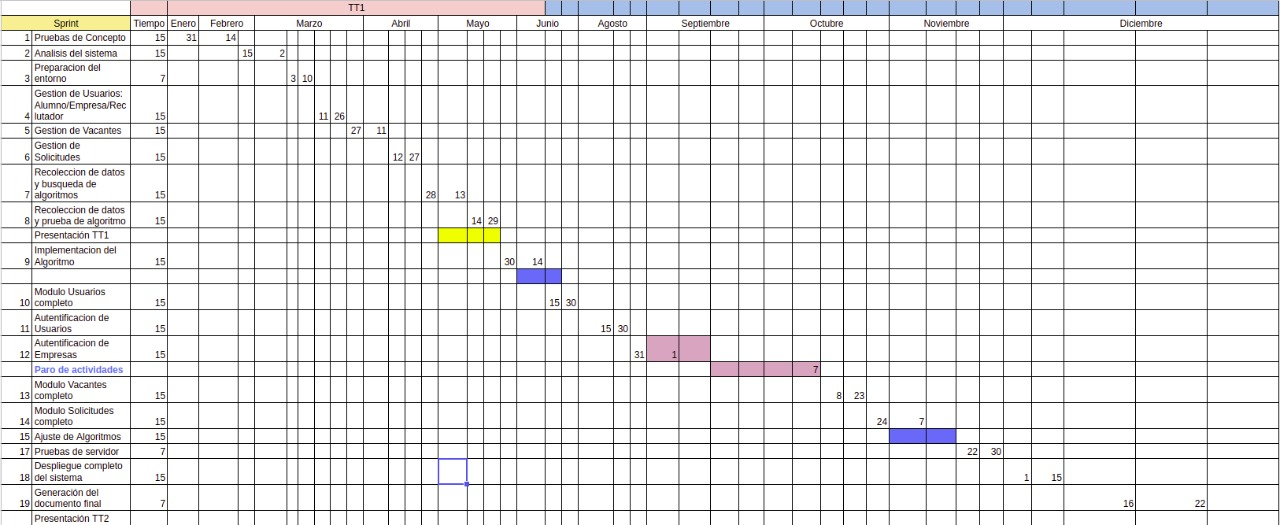
\includegraphics[width=.8\textwidth]{desarrollo/imagenes/cronograma.png}
    \end{center}
    \caption{Cronograma para Trabajo Terminal II.}
    \label{mark:top}
\end{figure}
 \clearpage

\subsection{Algoritmo de Recomendación}
En esta sección explicaremos  el desarrollo e implementación del algoritmo de recomendación, el cual se trabajó con el en la mayor parte de \textbf{Trabajo Terminal II}\\
\newline
Para el desarrollo del algoritmo se tuvo que analizar el problema desde diferentes perspectivas para encontrar un acercamiento del problema en el cual se involucraron coherentemente las características que el sistema ofrece a los candidatos en su perfil y a los reclutadores al ofertar una nueva vacante de manera que se puedan traducir, transformar y comparar la información de los candidatos y las vacantes en igualdad de condiciones y así ofrecer opciones de vacantes acordes al perfil de cada candidato. \\
\newline
En este apartado se describirán las opciones que se contemplaron para crear un algoritmo que se ajustará a las necesidades que tiene el sistema y que pudiese ser implementado con la información que se espera tener en el sistema para generar resultados de manera orgánica a los usuarios de la misma.
\subsubsection{Entradas}
El sistema fue planeado para guardar en el perfil del candidato las características que le interesan a los reclutadores de un candidato. Mientras que para guardar la información de las vacantes se inspiró el sistema en los formatos con los que ya cuenta la gestión de bolsa de trabajo actual para publicar nuevas vacantes en el boletín, por lo que la mayoría de sus características se rescataron o adaptaron para ser funcionales en los formularios que el sistema ofrece a los reclutadores para publicar una vacante con el máximo posible de información para que los candidatos puedan decidir si es conveniente para ellos o no. Tomando esto en cuenta se tiene que el sistema almacena la información de candidatos y vacantes como se muestra en la siguiente lista:

\begin{itemize}
    \item Candidato:
    \begin{itemize}
        \item Nombre
        \item Habilidades
        \item HIstorial académico
        \item Idiomas que domina 
        \item Objetivos profesionales 
        \item Experiencia profesional
        \item Curriculum vitae
        \item Residencia
        \item Métodos de contacto
        \item Salario deseado
        \item Modalidad de trabajo deseada
    \end{itemize} 
    \item Vacante:
    \begin{itemize}
        \item Puesto
        \item Número de plazas disponibles
        \item Ubicación
        \item Rango salarial ofrecido
        \item Perfil de escolar deseado
        \item Experiencia requerida
        \item Habilidades requeridas obligatoriamente y opcionalmente
        \item Idiomas requeridos 
        \item Tipo de contratación
        \item Horario laboral
        \item Modalidad de trabajo
        \item Descripción de la vacante
    \end{itemize} 
\end{itemize} 

Como se puede observar las características de candidatos y vacantes no son iguales por lo que se tuvo que comparar cuales son las características que comparten los candidatos y las vacantes y que podrían ser un diferenciador para decidir si una vacante es apta para un candidato o no. Las características en común que se encontraron son las siguientes:
\begin{itemize}
    \item Habilidades
    \item Idiomas
    \item Experiencia laboral
    \item Rango salarial
    \item Modalidad de trabajo
    \item Perfil académico
\end{itemize} 
Por lo que inicialmente se decidió empezar a  trabajar con esta información y buscar algún método con el cual se pudieran explotar estas características en común entre los candidatos y las vacantes.\\
\newline
Como se  ve en la comparación y se puede deducir, las habilidades solicitadas por la vacante puede ser el primer filtro por el cual se puede encontrar un candidato que se ajuste al perfil que se busca en la vacante, por lo que nuestros esfuerzos se centraron inicialmente en encontrar un algoritmo que hiciera uso de las habilidades como medio principal para identificar las vacantes que sean aptas para un candidato.

\subsubsection{Algoritmos candidatos}
\textbf{Ontologías}\\
\newline

Al definir cuales son las posibles entradas que el algoritmo puede tener basándonos en la información que el sistema guarda de las entidades entre las cuales se pretende encontrar una similitud, se detectó que la característica principal que tienen ambas entidades son las Habilidades. Por lo que primero se realizó un acercamiento en el cuál se aprovechará solamente de esta característica de las entidades que se analizarán, la primera opción que se encontró fue el uso de las ontologías. \\
\newline

La Ontología es una antigua disciplina que en sentido filosófico, se define como un esquema específico de categorías que refleja una visión específica del mundo. Desde el punto de vista informático las ontologías  son  teorías  que  especifican  un  vocabulario  relativo  a un  cierto  dominio.  Este  vocabulario  define  entidades,  clases, propiedades,  predicados,  funciones  y  las  relaciones  entre estos componentes. Las   ontologías   favorecen   la   comunicación   entre   personas,organizaciones    y    aplicaciones    porque    proporcionan    una comprensión  común  de  un  dominio,  de  modo  que  se  eliminan confusiones   conceptuales   y   terminológicas. \\
\newline

Las  ontologías  también  sirven  para  conseguir  que  los sistemas se operen  mutuamente.  Dos  sistemas  son  interoperables  si  pueden  trabajar  conjuntamente  de  una  forma automática, sin esfuerzo por parte del usuario. Por ejemplo, dos teléfonos móviles de distintos fabricantes y abonados a diferentes  compañías  telefónicas  inter-operan  para  que  los usuarios   puedan   hablar   entre   sí.   En   el   campo   de   la informática, las ontologías sirven para traducir los términos usados  por  una  aplicación  a  otra. Las ontologías resultan muy útiles para facilitar el razonamiento automático, es decir, sin intervención humana. Partiendo de unas reglas  de  inferencia,  un  motor  de  razonamiento  puede  usar  los datos  de  las  ontologías  para  inferir  conclusiones  de  ellos.  \\
\newline

Tomando en cuenta lo anterior se buscó diseñar e implementar una ontología que permitiera definir los posibles temas, campos y aplicaciones de conocimientos que las empresas que representan los reclutadores pudieran llegar a necesitar de candidatos registrados en el sistema y haciendo uso de esta ontología se pudieran clasificar a los candidatos para encontrar a los que mejor se adaptaran a los requerimientos que solicita cada vacante. \\
\newline

Inicialmente se realizó una investigación de cómo se estructura y define una ontología para diseñar una ontología que sea coherente con la información de la base de datos y así prevenir el que se necesite desarrollar más software del necesario para mantener en funcionamiento el análisis léxico de las vacantes agregadas al sistema. La primera propuesta de ontología fue enfocada a vacantes que se tenían de prueba y de ellas se obtuvieron las posibles ramas y hojas que componen a la ontología, la ontología resultante fue la que se muestra en la siguiente imagen.

\begin{figure}[H]
    \begin{center}
        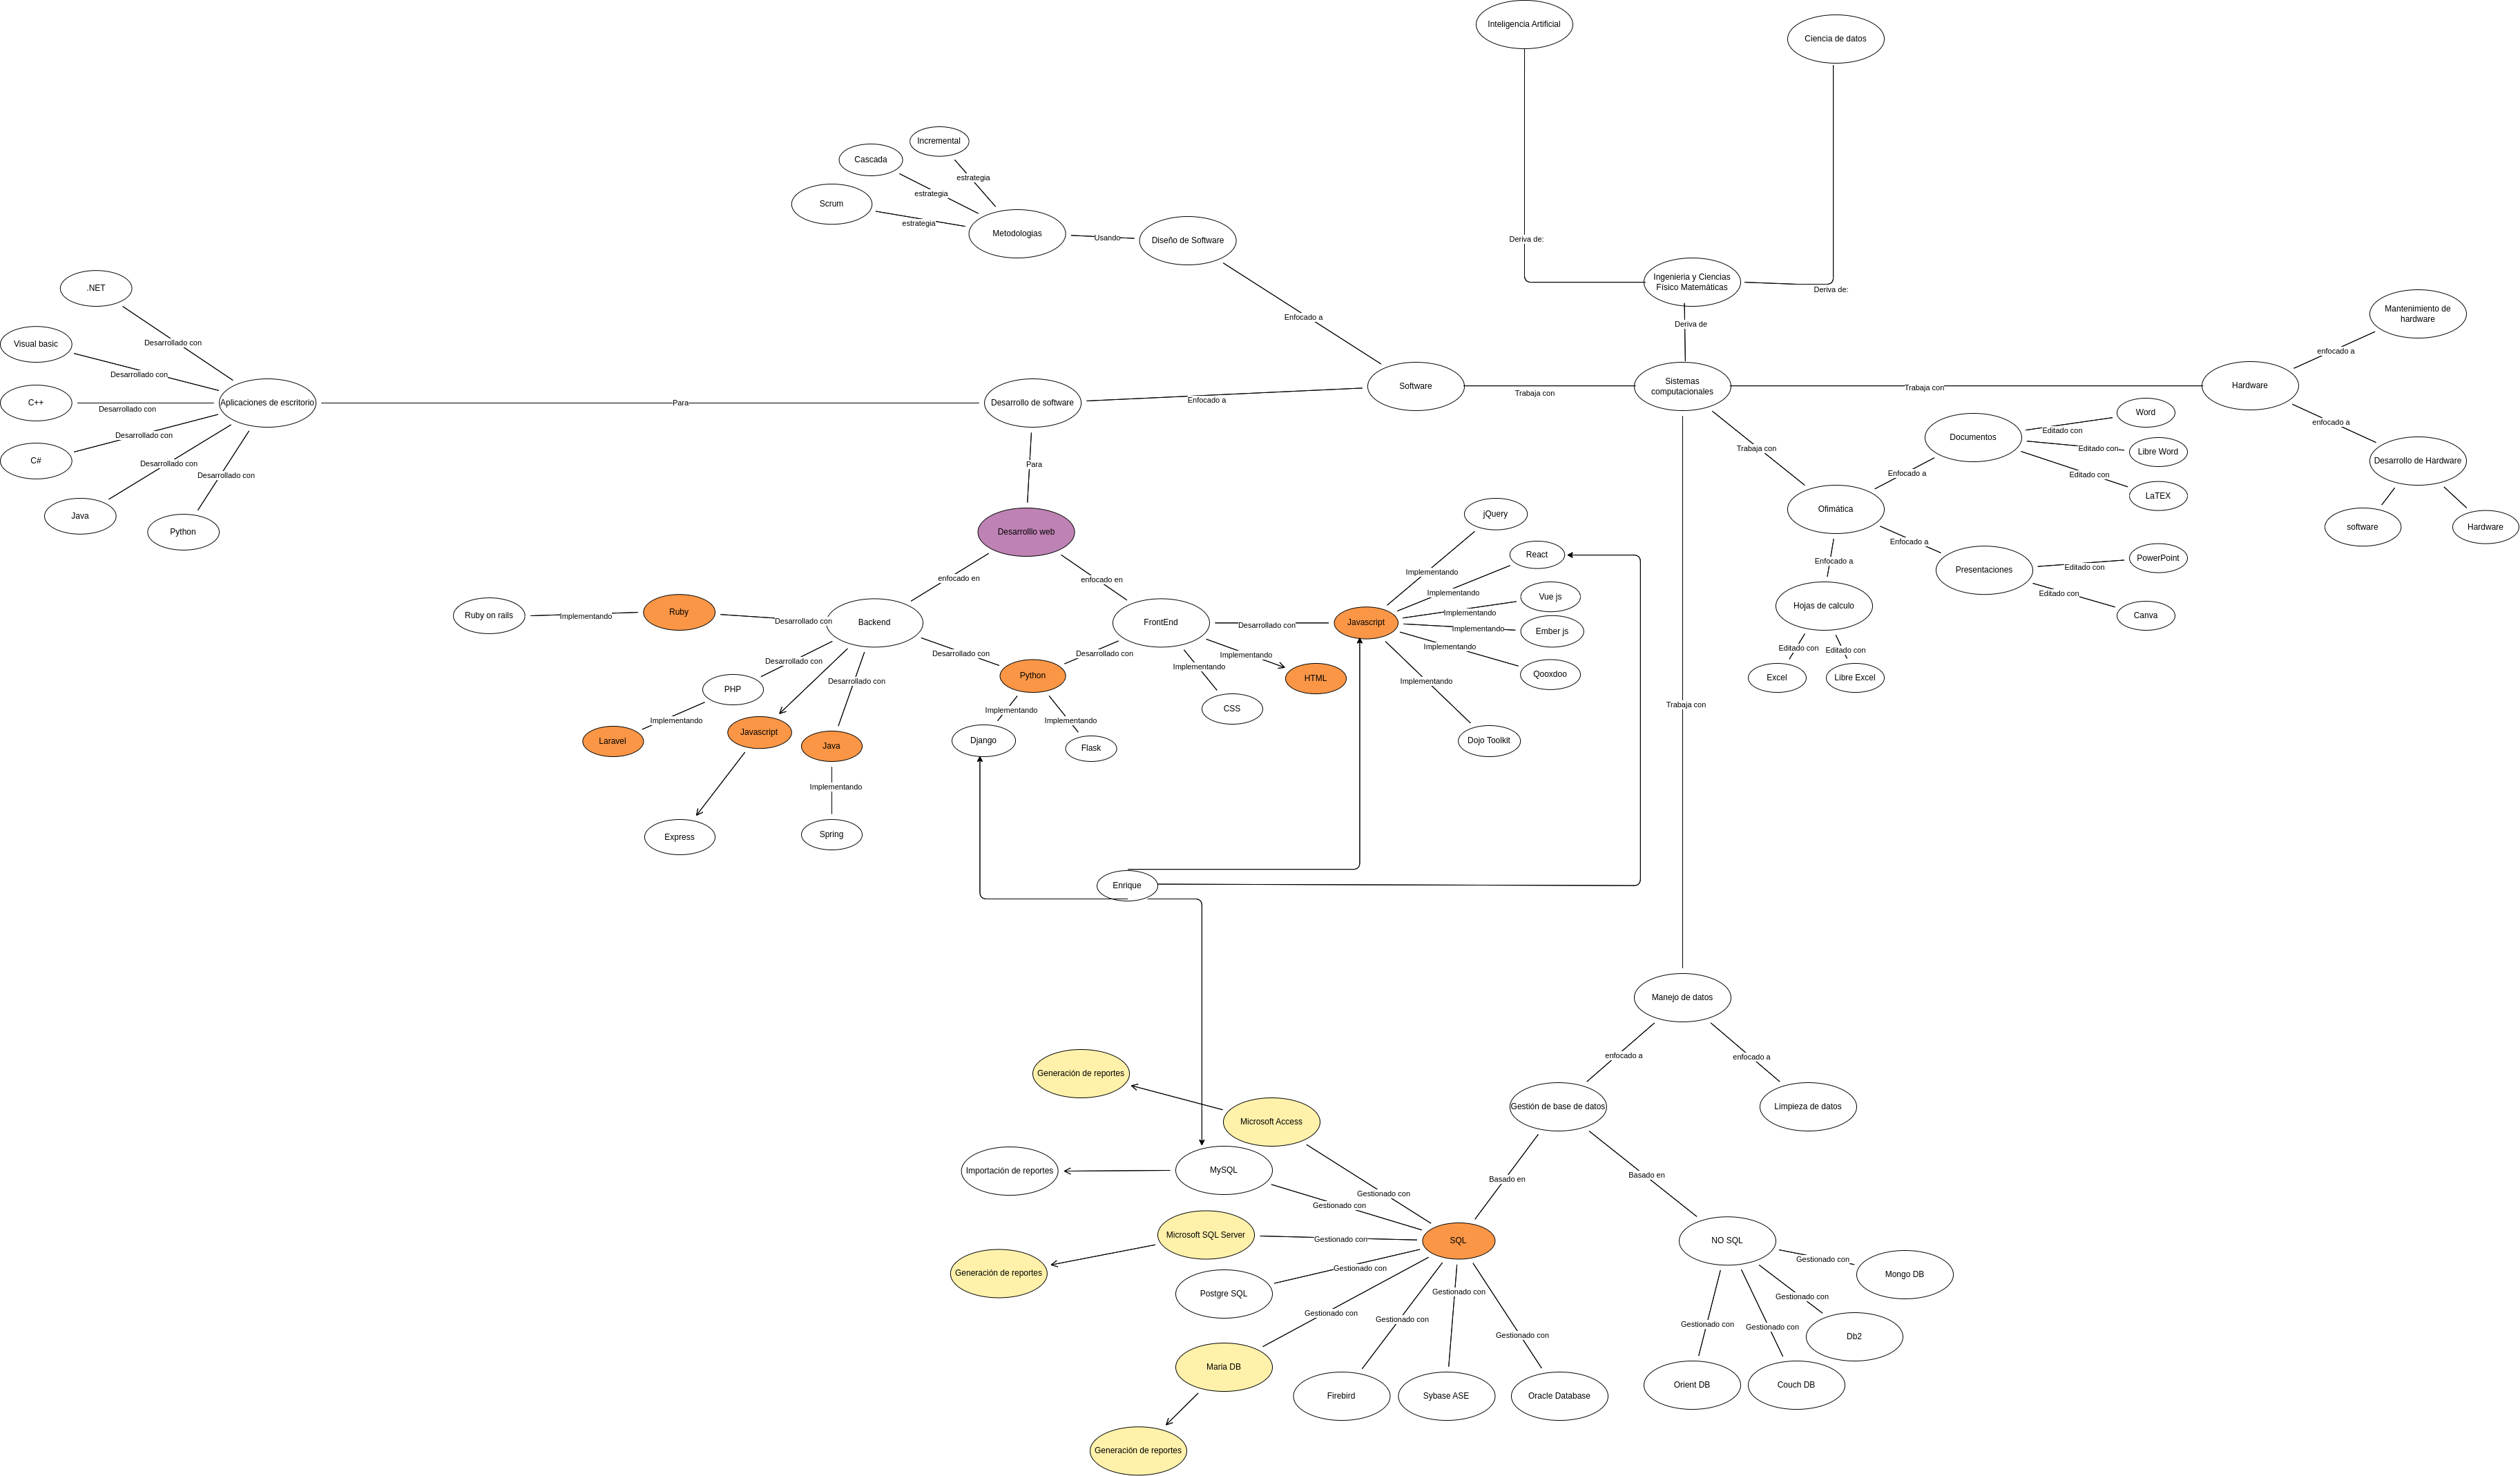
\includegraphics[width=.8\textwidth]{desarrollo/imagenes/Ontologia.png}
    \end{center}
    \caption{Ontología propuesta.}
    \label{mark:top}
\end{figure}
 \clearpage

\subsection{Gestión del sistema}
Con base en el cronograma, para \textbf{Trabajo Terminal II}  se abordaron 7 sprints, de los cuales 6 estaban enfocados en el sistema.
\begin{itemize}
    \item \textbf{Sprint 10 Modulo Usuarios completo} tuvo como propósito desarrollar los casos de uso prioritarios de módulo de usuarios.
    Cada caso de uso fue redactado y posteriormente desarrollados por el equipo, dichos casos de uso se listan a continuación y el diagrama se muestra en la figura \ref{adcu:usr}.
    \begin{itemize}
        \item \refIdElem{USR-CU01}
        \item \refIdElem{USR-CU02}
        \item \refIdElem{USR-CU02.1}
        \item \refIdElem{USR-CU02.2}
        \item \refIdElem{USR-CU02.3}
        \item \refIdElem{USR-CU02.4}
        \item \refIdElem{USR-CU02.5}
        \item \refIdElem{USR-CU02.6}
        \item \refIdElem{USR-CU02.7}
        \item \refIdElem{USR-CU03}
        \item \refIdElem{USR-CU03.1}
        \item \refIdElem{USR-CU03.2}
        \item \refIdElem{USR-CU03.3}
        \item \refIdElem{USR-CU04}
        \item \refIdElem{USR-CU04.1}
        \item \refIdElem{USR-CU04.2}
        \item \refIdElem{USR-CU04.3}
        \item \refIdElem{USR-CU05}
        \item \refIdElem{USR-CU06}
        \item \refIdElem{USR-CU06.1}
        \item \refIdElem{USR-CU06.2}
        \item \refIdElem{USR-CU06.3}
    \end{itemize} 

    Como ya se ha explicado, el Modulo de Usuarios tiene como objetivo cubrir los requerimientos esenciales para las cuentas de cada actor que interactúa con el sistema.
    para \textbf{Trabajo Terminal II} se tomaron como prioridad implementar los casos de uso del actor \textbf{Candidato} los cuales cubren la gestión de su perfil dentro del sistema.
    Ya que es necesario visualizar los archivos PDF's se implementó la visualización  y almacenamiento de dichos archivos.
    

    \item \textbf{Sprint 11 y 12 Autentificación de Usuarios y Autentificación de Empresas} estos dos sprints tuvieron como propósito desarrollar los casos de uso prioritarios para la autentificación de reclutadores y empresas dentro del sistema
    Cada caso de uso fue redactado y posteriormente desarrollado por el equipo, dichos casos de uso se listan a continuación y el diagrama se muestra en la figura \ref{adcu:admn}.
    \begin{itemize}
        \item \refIdElem{ADMN-CU02}
        \item \refIdElem{ADMN-CU02.1}
        \item \refIdElem{ADMN-CU02.2}
        \item \refIdElem{ADMN-CU02.3}
        \item \refIdElem{ADMN-CU03}
        \item \refIdElem{ADMN-CU04}
    \end{itemize} 
    En este sprint se implemento la generación de contraseñas dinámicas para la cuentas de los reclutadores y colaboradores dentro del sistema, cada cuenta que es creada se le asigna una contraseña provisional, la cual genera automáticamente el sistema cuyo formato cumple con la regla de negocio \refIdElem{RN-N006}.
    

    \item \textbf{Sprint 13 y 14 Modulo Vacantes y Solicitudes} en estos dos sprits se tuvieron juntas con el licenciado José Francisco Serrano García donde se reajustaron requerimientos sobre la consulta y de solicitudes y vacantes para todos los 
    usuarios dentro del sistema los cuales fueron:
    \begin{itemize}
        \item Todos cualquier usuario podrá consultar información que se tenga sobre las empresas registradas.
        \item Un reclutador podrá consultar unicamente el perfil de los candidatos que se hayan postulado a sus vacantes.
        \item Todas las pantallas deben de tener in titulo como contexto del negocio.
        \item Toda sesión debe de indicar el tipo de actor con el que el usuario ingreso.
        \item Se debe validar cada vacante que desea ser publicada en el sistema antes que que cualquier candidato la pueda consultar y si es necesario se debe de mandar observaciones al reclutador que haya registrado la vacante.
    \end{itemize} 

    Cada caso de uso fue corregido y actualizado en el sistema, el diagrama se muestra en la figura \ref{adcu:vct}.
    \begin{itemize}
        \item \refIdElem{PST-CU01}
        \item \refIdElem{PST-CU01.1}
        \item \refIdElem{PST-CU01.2}
        \item \refIdElem{VCT-CU01}
        \item \refIdElem{VCT-CU02} 
        \item \refIdElem{VCT-CU02.1} 
        \item \refIdElem{VCT-CU03}
        \item \refIdElem{VCT-CU04}
    \end{itemize} 

    El hecho que se necesitara de una gestión de observaciones para las vacantes necesito agregar una tabla nueva en el sistema, la cual tiene como objetivo guardar la relación entre la observación, el quien la realizó y para quien va la obsercación.
    \begin{figure}[H]
        \begin{center}
            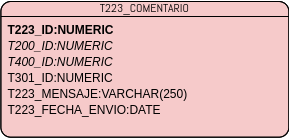
\includegraphics[width=.4\textwidth]{desarrollo/imagenes/nueva.png}
        \end{center}
        \caption{Entidad para la gestión de observaciones.}
        \label{mark:top}
    \end{figure}

\end{itemize} 

